\FloatBarrier

% Problema \getNumeroProblema
\begin{table}[htbp]
  \centering
  \renewcommand{\arraystretch}{1.5}
  \begin{tabular}{|>{\raggedright\arraybackslash}p{7.5cm}|>{\raggedright\arraybackslash}p{7.5cm}|}
    \hline
    \rowcolor{green!30}
    \multicolumn{2}{|c|}{\textbf{Problema \getNumeroProblema}} \\
    \hline
    \textbf{Descrizione} & Nella pagina "I Miei Appunti", una volta cliccato sul tab "Appunti Salvati", viene presentata una pagina completamente diversa da quella che mi aspetterei. Analogamente cliccando sul tab "Appunti della Community". \\
    \hline
    \textbf{Pagina del sito} & Dashboard - I Miei Appunti \\
    \hline
    \textbf{Principi violati} & 2 (Adeguare il sistema al mondo reale); 4 (Assicurare consistenza) \\
    \hline
    \textbf{Grado di severità} & 2 (Problema secondario) \\
    \hline
    \textbf{Nome del valutatore} & Legati \\
    \hline
  \end{tabular}
\end{table}

% Problema \getNumeroProblema
\begin{table}[htbp]
  \centering
  \renewcommand{\arraystretch}{1.5}
  \begin{tabular}{|>{\raggedright\arraybackslash}p{7.5cm}|>{\raggedright\arraybackslash}p{7.5cm}|}
    \hline
    \rowcolor{green!30}
    \multicolumn{2}{|c|}{\textbf{Problema \getNumeroProblema}} \\
    \hline
    \textbf{Descrizione} & Durante il caricamento di un nuovo file nella sezione appunti, il titolo "Upload" è in inglese. \\
    \hline
    \textbf{Pagina del sito} & Dashboard - I Miei Appunti - Caricamento File \\
    \hline
    \textbf{Principi violati} & 2 (Adeguare il sistema al mondo reale); 4 (Assicurare consistenza) \\
    \hline
    \textbf{Grado di severità} & 2 (Problema secondario) \\
    \hline
    \textbf{Screen} &
    \vspace{10pt}
    \hspace*{\fill}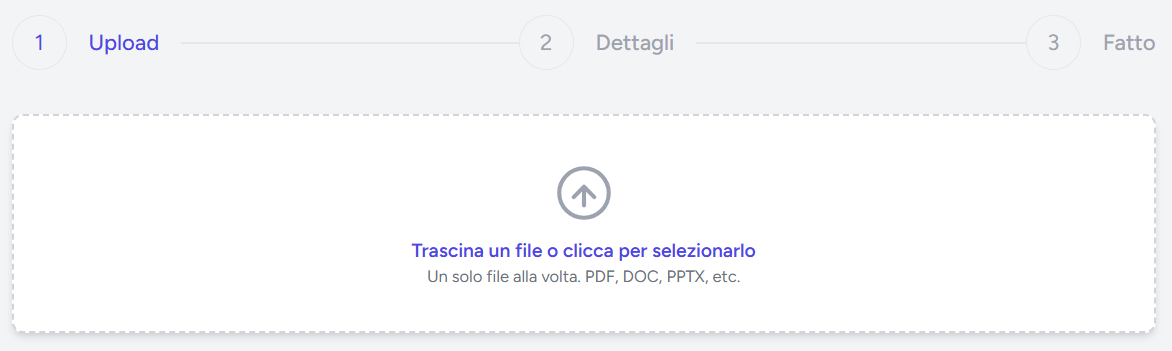
\includegraphics[width=6.5cm]{Screenshots/foglio2/problema003.png}\hspace*{\fill}
    \vspace{10pt}
    \\
    \hline
    \textbf{Nome del valutatore} & Legati, Rinaldi, Kharef \\
    \hline
  \end{tabular}
\end{table}

% Problema \getNumeroProblema
\begin{table}[htbp]
  \centering
  \renewcommand{\arraystretch}{1.5}
  \begin{tabular}{|>{\raggedright\arraybackslash}p{7.5cm}|>{\raggedright\arraybackslash}p{7.5cm}|}
    \hline
    \rowcolor{green!30}
    \multicolumn{2}{|c|}{\textbf{Problema \getNumeroProblema}} \\
    \hline
    \textbf{Descrizione} & Durante il caricamento di un nuovo file nella sezione appunti, il titolo "Fatto" è un po' generico. \\
    \hline
    \textbf{Pagina del sito} & Dashboard - I Miei Appunti - Caricamento File \\
    \hline
    \textbf{Principi violati} & 2 (Adeguare il sistema al mondo reale); 5 (Riconoscimento piuttosto che uso della memoria dell’utente) \\
    \hline
    \textbf{Grado di severità} & 0 (Non è un problema di usabilità) \\
    \hline
    \textbf{Screen} &
    \vspace{10pt}
    \hspace*{\fill}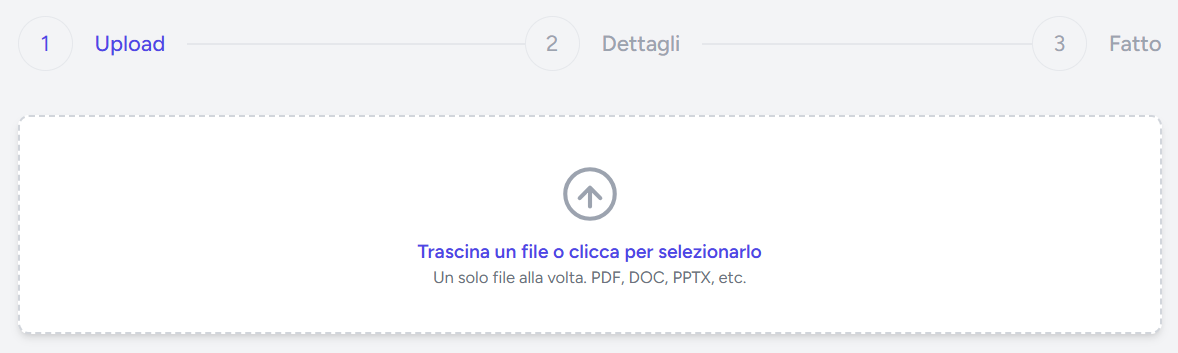
\includegraphics[width=6.5cm]{Screenshots/foglio2/problema004.png}\hspace*{\fill}
    \vspace{10pt}
    \\
    \hline
    \textbf{Nome del valutatore} & Legati \\
    \hline
  \end{tabular}
\end{table}

% Problema \getNumeroProblema
\begin{table}[htbp]
  \centering
  \renewcommand{\arraystretch}{1.5}
  \begin{tabular}{|>{\raggedright\arraybackslash}p{7.5cm}|>{\raggedright\arraybackslash}p{7.5cm}|}
    \hline
    \rowcolor{green!30}
    \multicolumn{2}{|c|}{\textbf{Problema \getNumeroProblema}} \\
    \hline
    \textbf{Descrizione} & Durante il caricamento di un nuovo file nella sezione appunti, la modifica dei valori nella sezione "Dettagli" implica un refresh visibile del contenuto. \\
    \hline
    \textbf{Pagina del sito} & Dashboard - I Miei Appunti - Caricamento File \\
    \hline
    \textbf{Principi violati} & 4 (Assicurare consistenza) \\
    \hline
    \textbf{Grado di severità} & 3 (Problema rilevante) \\
    \hline
    \textbf{Nome del valutatore} & Legati, Kharef \\
    \hline
  \end{tabular}
\end{table}

% Problema \getNumeroProblema
\begin{table}[htbp]
  \centering
  \renewcommand{\arraystretch}{1.5}
  \begin{tabular}{|>{\raggedright\arraybackslash}p{7.5cm}|>{\raggedright\arraybackslash}p{7.5cm}|}
    \hline
    \rowcolor{green!30}
    \multicolumn{2}{|c|}{\textbf{Problema \getNumeroProblema}} \\
    \hline
    \textbf{Descrizione} & Durante il caricamento di un nuovo file nella sezione appunti, i messaggi di errore nella sezione "Dettagli" sono scritti in inglese. \\
    \hline
    \textbf{Pagina del sito} & Dashboard - I Miei Appunti - Caricamento File \\
    \hline
    \textbf{Principi violati} & 2 (Adeguare il sistema al mondo reale); 4 (Assicurare consistenza); 9 (Permettere all’utente di correggere gli errori e non solo di rilevarli) \\
    \hline
    \textbf{Grado di severità} & 2 (Problema secondario) \\
    \hline
    \textbf{Screen} &
    \vspace{10pt}
    \hspace*{\fill}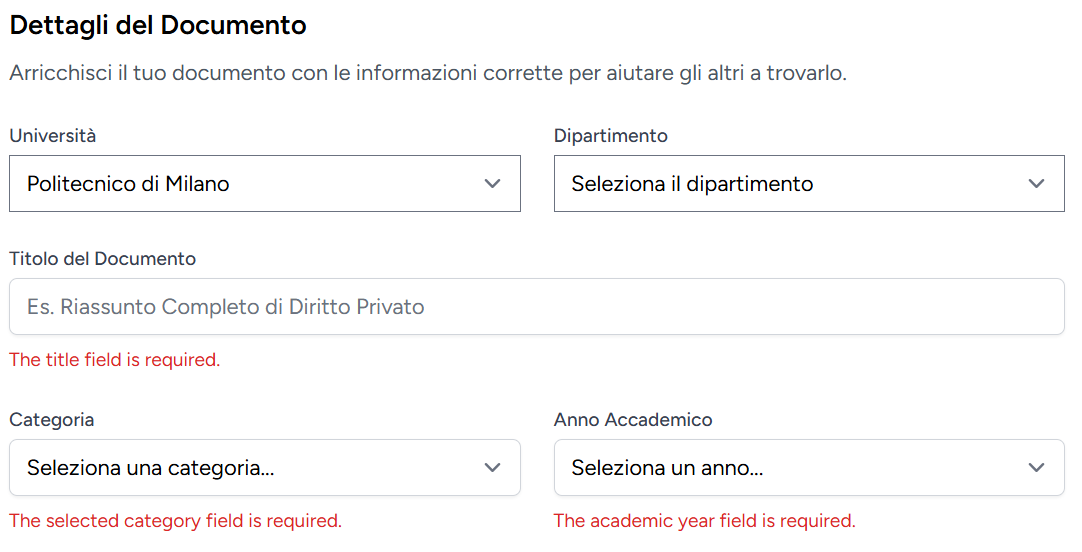
\includegraphics[width=6.5cm]{Screenshots/foglio2/problema006.png}\hspace*{\fill}
    \vspace{10pt}
    \\
    \hline
    \textbf{Nome del valutatore} & Legati, Rinaldi \\
    \hline
  \end{tabular}
\end{table}

% Problema \getNumeroProblema
\begin{table}[htbp]
  \centering
  \renewcommand{\arraystretch}{1.5}
  \begin{tabular}{|>{\raggedright\arraybackslash}p{7.5cm}|>{\raggedright\arraybackslash}p{7.5cm}|}
    \hline
    \rowcolor{green!30}
    \multicolumn{2}{|c|}{\textbf{Problema \getNumeroProblema}} \\
    \hline
    \textbf{Descrizione} & Durante il caricamento di un nuovo file nella sezione appunti, i messaggi di errore nella sezione "Dettagli" non scompaiono dopo che il contenuto del campo è stato modificato (e validato). \\
    \hline
    \textbf{Pagina del sito} & Dashboard - I Miei Appunti - Caricamento File \\
    \hline
    \textbf{Principi violati} & 1 (Far vedere lo stato del sistema); 8 (Prevenire gli errori) \\
    \hline
    \textbf{Grado di severità} & 3 (Problema rilevante) \\
    \hline
    \textbf{Screen} &
    \vspace{10pt}
    \hspace*{\fill}
\includegraphics[width=6.5cm]{Screenshots/foglio2/problema007.png}\hspace*{\fill}
    \vspace{10pt}
    \\
    \hline
    \textbf{Nome del valutatore} & Legati \\
    \hline
  \end{tabular}
\end{table}

% Problema \getNumeroProblema
\begin{table}[htbp]
  \centering
  \renewcommand{\arraystretch}{1.5}
  \begin{tabular}{|>{\raggedright\arraybackslash}p{7.5cm}|>{\raggedright\arraybackslash}p{7.5cm}|}
    \hline
    \rowcolor{green!30}
    \multicolumn{2}{|c|}{\textbf{Problema \getNumeroProblema}} \\
    \hline
    \textbf{Descrizione} & Nella pagina "I Miei Appunti" e "I Miei Materiali", se non sono presenti cartelle e file compare il messaggio "no folder trovato", un mix di italiano e inglese. \\
    \hline
    \textbf{Pagina del sito} & Dashboard - I Miei Appunti - I Miei Materiali \\
    \hline
    \textbf{Principi violati} & 2 (Adeguare il sistema al mondo reale); 4 (Assicurare consistenza) \\
    \hline
    \textbf{Grado di severità} & 2 (Problema secondario) \\
    \hline
    \textbf{Screen} &
    \vspace{10pt}
    \hspace*{\fill}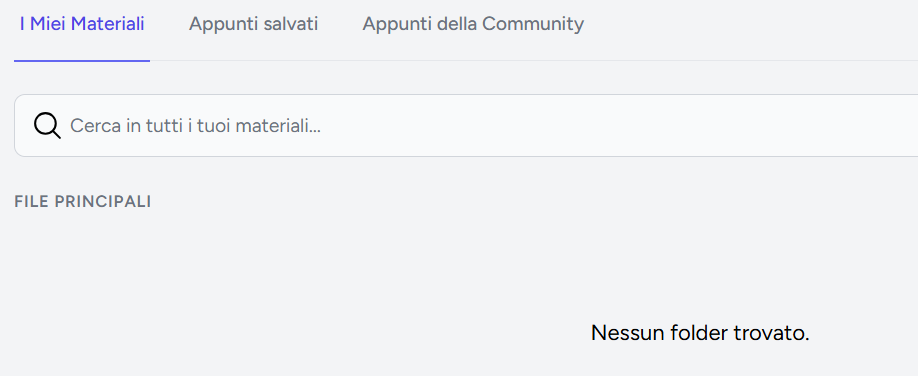
\includegraphics[width=6.5cm]{Screenshots/foglio2/problema008.png}\hspace*{\fill}
    \vspace{10pt}
    \\
    \hline
    \textbf{Nome del valutatore} & Legati, Rinaldi \\
    \hline
  \end{tabular}
\end{table}

% Problema \getNumeroProblema
\begin{table}[htbp]
  \centering
  \renewcommand{\arraystretch}{1.5}
  \begin{tabular}{|>{\raggedright\arraybackslash}p{7.5cm}|>{\raggedright\arraybackslash}p{7.5cm}|}
    \hline
    \rowcolor{green!30}
    \multicolumn{2}{|c|}{\textbf{Problema \getNumeroProblema}} \\
    \hline
    \textbf{Descrizione} & Nella pagina "Mostra Documento", la sezione "Caricato da" (l'autore) non è cliccabile. \\
    \hline
    \textbf{Pagina del sito} & Dashboard - I Miei Appunti - Mostra Documento \\
    \hline
    \textbf{Principi violati} & 5 (Riconoscimento piuttosto che uso della memoria dell’utente); 6 (Assicurare flessibilità ed efficienza d’uso) \\
    \hline
    \textbf{Grado di severità} & 2 (Problema secondario) \\
    \hline
    \textbf{Nome del valutatore} & Legati, Kharef \\
    \hline
  \end{tabular}
\end{table}

% Problema \getNumeroProblema
\begin{table}[htbp]
  \centering
  \renewcommand{\arraystretch}{1.5}
  \begin{tabular}{|>{\raggedright\arraybackslash}p{7.5cm}|>{\raggedright\arraybackslash}p{7.5cm}|}
    \hline
    \rowcolor{green!30}
    \multicolumn{2}{|c|}{\textbf{Problema \getNumeroProblema}} \\
    \hline
    \textbf{Descrizione} & Nella pagina "Mostra Documento" e sotto la voce "Corso", la voce non è cliccabile. \\
    \hline
    \textbf{Pagina del sito} & Dashboard - I Miei Appunti - Mostra Documento \\
    \hline
    \textbf{Principi violati} & 5 (Riconoscimento piuttosto che uso della memoria dell’utente); 6 (Assicurare flessibilità ed efficienza d’uso) \\
    \hline
    \textbf{Grado di severità} & 2 (Problema secondario) \\
    \hline
    \textbf{Nome del valutatore} & Legati \\
    \hline
  \end{tabular}
\end{table}

%----------------------------------------------------------------
\FloatBarrier

% Problema \getNumeroProblema
\begin{table}[htbp]
  \centering
  \renewcommand{\arraystretch}{1.5}
  \begin{tabular}{|>{\raggedright\arraybackslash}p{7.5cm}|>{\raggedright\arraybackslash}p{7.5cm}|}
    \hline
    \rowcolor{green!30}
    \multicolumn{2}{|c|}{\textbf{Problema \getNumeroProblema}} \\
    \hline
    \textbf{Descrizione} & Nella pagina ”Mostra Documento” e ”Commenti”, i commenti vengono visualizzati in un punto poco visibile. \\
    \hline
    \textbf{Pagina del sito} & Dashboard - I Miei Appunti - Mostra Documento \\
    \hline
    \textbf{Principi violati} & 5 (Riconoscimento piuttosto che uso della memoria dell’utente); 7 (Visualizzare tutte e sole le informazioni necessarie) \\
    \hline
    \textbf{Grado di severità} & 2 (Problema secondario) \\
    \hline
    \textbf{Nome del valutatore} & Legati, Kharef \\
    \hline
  \end{tabular}
\end{table}

% Problema \getNumeroProblema
\begin{table}[htbp]
  \centering
  \renewcommand{\arraystretch}{1.5}
  \begin{tabular}{|>{\raggedright\arraybackslash}p{7.5cm}|>{\raggedright\arraybackslash}p{7.5cm}|}
    \hline
    \rowcolor{green!30}
    \multicolumn{2}{|c|}{\textbf{Problema \getNumeroProblema}} \\
    \hline
    \textbf{Descrizione} & Nella pagina ”Esplora Appunti” e visualizzando gli appunti in una griglia, quando l'utente clicca sull'icona del documento, l'azione non funziona; è necessario cliccare il bordo della card per accedere. \\
    \hline
    \textbf{Pagina del sito} & Dashboard - Esplora Appunti \\
    \hline
    \textbf{Principi violati} & 5 (Riconoscimento piuttosto che uso della memoria dell’utente) \\
    \hline
    \textbf{Grado di severità} & 3 (Problema rilevante) \\
    \hline
    \textbf{Screen} &
    \vspace{10pt}
    \hspace*{\fill}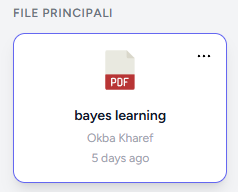
\includegraphics[width=6.5cm]{Screenshots/foglio3/problema63.png}\hspace*{\fill}
    \vspace{10pt}
    \\
    \hline
    \textbf{Nome del valutatore} & Legati, Kharef \\
    \hline
  \end{tabular}
\end{table}

% Problema \getNumeroProblema
\begin{table}[htbp]
  \centering
  \renewcommand{\arraystretch}{1.5}
  \begin{tabular}{|>{\raggedright\arraybackslash}p{7.5cm}|>{\raggedright\arraybackslash}p{7.5cm}|}
    \hline
    \rowcolor{green!30}
    \multicolumn{2}{|c|}{\textbf{Problema \getNumeroProblema}} \\
    \hline
    \textbf{Descrizione} & Nella pagina ”Esplora Appunti” e visualizzando gli appunti in una griglia, la data di caricamento del documento e l'università non sono visibili. \\
    \hline
    \textbf{Pagina del sito} & Dashboard - Esplora Appunti \\
    \hline
    \textbf{Principi violati} & 2 (Adeguare il sistema al mondo reale); 7 (Visualizzare tutte e sole le informazioni necessarie) \\
    \hline
    \textbf{Grado di severità} & 2 (Problema secondario) \\
    \hline
    \textbf{Nome del valutatore} & Legati, Kharef \\
    \hline
  \end{tabular}
\end{table}

% Problema \getNumeroProblema
\begin{table}[htbp]
  \centering
  \renewcommand{\arraystretch}{1.5}
  \begin{tabular}{|>{\raggedright\arraybackslash}p{7.5cm}|>{\raggedright\arraybackslash}p{7.5cm}|}
    \hline
    \rowcolor{green!30}
    \multicolumn{2}{|c|}{\textbf{Problema \getNumeroProblema}} \\
    \hline
    \textbf{Descrizione} & Nella pagina ”Esplora Appunti”, il pulsante ”Scarica” cambia aspetto a seconda del tipo di visualizzazione (lista o griglia). \\
    \hline
    \textbf{Pagina del sito} & Dashboard - Esplora Appunti \\
    \hline
    \textbf{Principi violati} & 4 (Assicurare consistenza) \\
    \hline
    \textbf{Grado di severità} & 1 (Problema accessorio) \\
    \hline
    \textbf{Nome del valutatore} & Legati \\
    \hline
  \end{tabular}
\end{table}

% Problema \getNumeroProblema
\begin{table}[htbp]
  \centering
  \renewcommand{\arraystretch}{1.5}
  \begin{tabular}{|>{\raggedright\arraybackslash}p{7.5cm}|>{\raggedright\arraybackslash}p{7.5cm}|}
    \hline
    \rowcolor{green!30}
    \multicolumn{2}{|c|}{\textbf{Problema \getNumeroProblema}} \\
    \hline
    \textbf{Descrizione} & Nella pagina ”Esplora Appunti”, il nome dell’utente che ha caricato il documento cambia aspetto a seconda del tipo di visualizzazione. \\
    \hline
    \textbf{Pagina del sito} & Dashboard - Esplora Appunti \\
    \hline
    \textbf{Principi violati} & 4 (Assicurare consistenza); 7 (Visualizzare tutte e sole le informazioni necessarie) \\
    \hline
    \textbf{Grado di severità} & 1 (Problema accessorio) \\
    \hline
    \textbf{Nome del valutatore} & Legati \\
    \hline
  \end{tabular}
\end{table}

% Problema \getNumeroProblema
\begin{table}[htbp]
  \centering
  \renewcommand{\arraystretch}{1.5}
  \begin{tabular}{|>{\raggedright\arraybackslash}p{7.5cm}|>{\raggedright\arraybackslash}p{7.5cm}|}
    \hline
    \rowcolor{green!30}
    \multicolumn{2}{|c|}{\textbf{Problema \getNumeroProblema}} \\
    \hline
    \textbf{Descrizione} & Nella pagina ”Esplora Appunti”, i pollici sembrano bottoni ma non fanno nulla. \\
    \hline
    \textbf{Pagina del sito} & Dashboard - Esplora Appunti \\
    \hline
    \textbf{Principi violati} & 5 (Riconoscimento piuttosto che uso della memoria dell’utente) \\
    \hline
    \textbf{Grado di severità} & 1 (Problema accessorio) \\
    \hline
    \textbf{Nome del valutatore} & Legati \\
    \hline
  \end{tabular}
\end{table}

% Problema \getNumeroProblema
\begin{table}[htbp]
  \centering
  \renewcommand{\arraystretch}{1.5}
  \begin{tabular}{|>{\raggedright\arraybackslash}p{7.5cm}|>{\raggedright\arraybackslash}p{7.5cm}|}
    \hline
    \rowcolor{green!30}
    \multicolumn{2}{|c|}{\textbf{Problema \getNumeroProblema}} \\
    \hline
    \textbf{Descrizione} & Nella pagina ”Sbobinatore AI”, il microfono del titolo sembra un bottone, ma non fa nulla. \\
    \hline
    \textbf{Pagina del sito} & Dashboard - Sbobinatore AI \\
    \hline
    \textbf{Principi violati} & 4 (Assicurare consistenza); 5 (Riconoscimento piuttosto che uso della memoria dell’utente) \\
    \hline
    \textbf{Grado di severità} & 1 (Problema accessorio) \\
    \hline
    \textbf{Screen} &
    \vspace{10pt}
    \hspace*{\fill}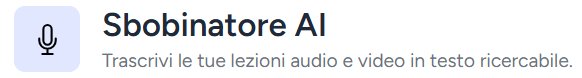
\includegraphics[width=6.5cm]{Screenshots/foglio2/problema018.png}\hspace*{\fill}
    \vspace{10pt}
    \\
    \hline
    \textbf{Nome del valutatore} & Legati \\
    \hline
  \end{tabular}
\end{table}

% Problema \getNumeroProblema
\begin{table}[htbp]
  \centering
  \renewcommand{\arraystretch}{1.5}
  \begin{tabular}{|>{\raggedright\arraybackslash}p{7.5cm}|>{\raggedright\arraybackslash}p{7.5cm}|}
    \hline
    \rowcolor{green!30}
    \multicolumn{2}{|c|}{\textbf{Problema \getNumeroProblema}} \\
    \hline
    \textbf{Descrizione} & Nella pagina ”Sbobinatore AI”, il bottone ”NUOVA TRASCRIZIONE” si trova in un punto poco funzionale. \\
    \hline
    \textbf{Pagina del sito} & Dashboard - Sbobinatore AI \\
    \hline
    \textbf{Principi violati} & 5 (Riconoscimento piuttosto che uso della memoria dell’utente) \\
    \hline
    \textbf{Grado di severità} & 1 (Problema accessorio) \\
    \hline
    \textbf{Screen} &
    \vspace{10pt}
    \hspace*{\fill}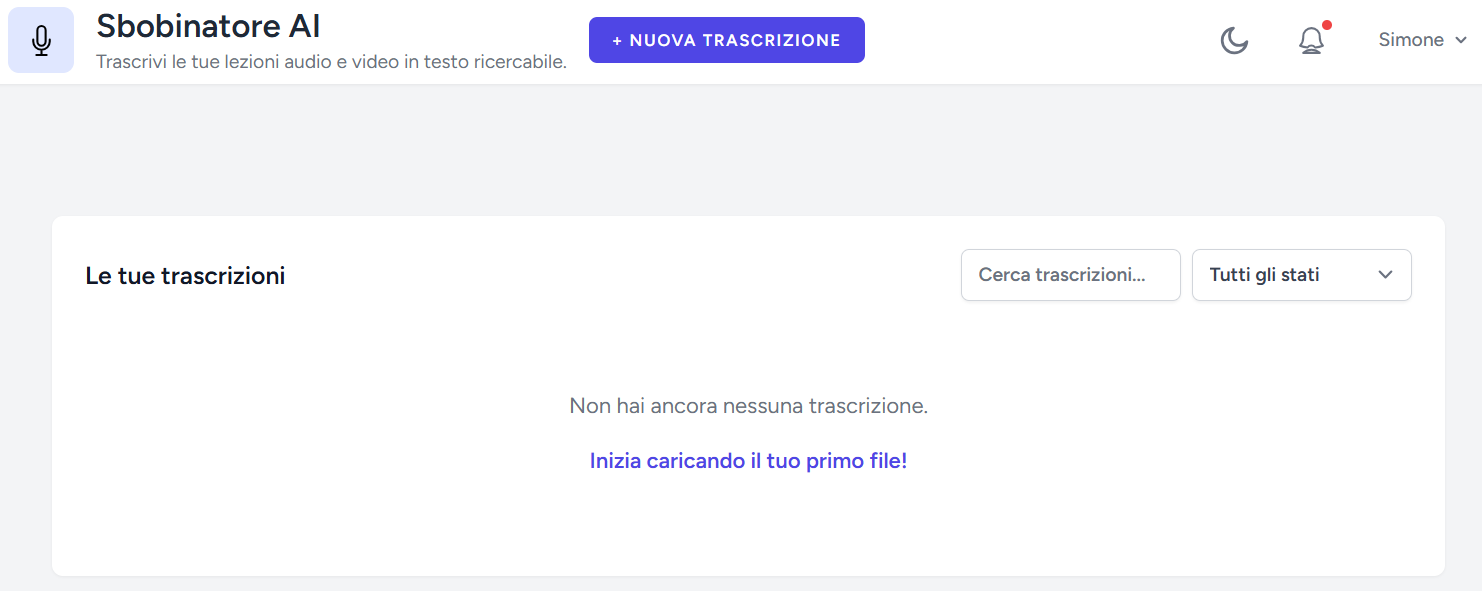
\includegraphics[width=6.5cm]{Screenshots/foglio2/problema019.png}\hspace*{\fill}
    \vspace{10pt}
    \\
    \hline
    \textbf{Nome del valutatore} & Legati \\
    \hline
  \end{tabular}
\end{table}

% Problema \getNumeroProblema
\begin{table}[htbp]
  \centering
  \renewcommand{\arraystretch}{1.5}
  \begin{tabular}{|>{\raggedright\arraybackslash}p{7.5cm}|>{\raggedright\arraybackslash}p{7.5cm}|}
    \hline
    \rowcolor{green!30}
    \multicolumn{2}{|c|}{\textbf{Problema \getNumeroProblema}} \\
    \hline
    \textbf{Descrizione} & Nella pagina ”Sbobinatore AI”, se non ho trascrizioni caricate mi viene proposto di farlo con un testo al centro della pagina ma è già presente il bottone. \\
    \hline
    \textbf{Pagina del sito} & Dashboard - Sbobinatore AI \\
    \hline
    \textbf{Principi violati} & 4 (Assicurare consistenza); 7 (Visualizzare tutte e sole le informazioni necessarie) \\
    \hline
    \textbf{Grado di severità} & 1 (Problema accessorio) \\
    \hline
    \textbf{Screen} &
    \vspace{10pt}
    \hspace*{\fill}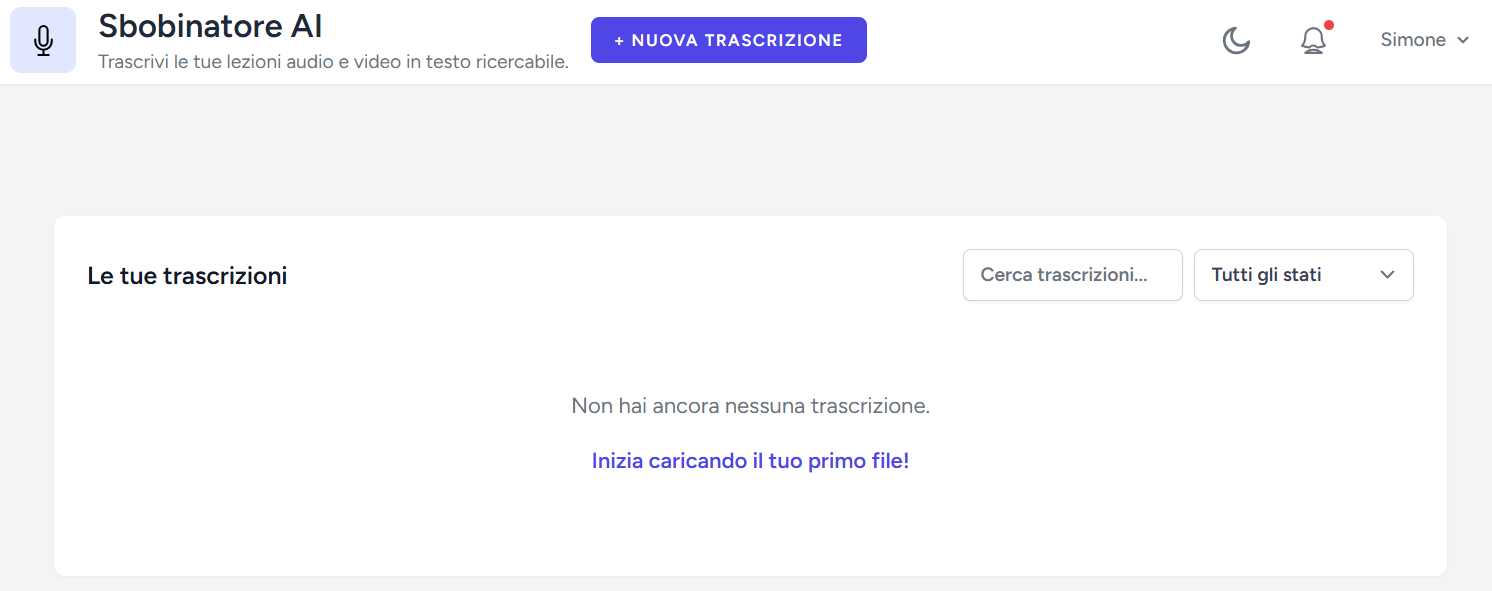
\includegraphics[width=6.5cm]{Screenshots/foglio2/problema020.png}\hspace*{\fill}
    \vspace{10pt}
    \\
    \hline
    \textbf{Nome del valutatore} & Legati \\
    \hline
  \end{tabular}
\end{table}

% Problema \getNumeroProblema
\begin{table}[htbp]
  \centering
  \renewcommand{\arraystretch}{1.5}
  \begin{tabular}{|>{\raggedright\arraybackslash}p{7.5cm}|>{\raggedright\arraybackslash}p{7.5cm}|}
    \hline
    \rowcolor{green!30}
    \multicolumn{2}{|c|}{\textbf{Problema \getNumeroProblema}} \\
    \hline
    \textbf{Descrizione} & Nella pagina ”AudioNote AI”, l’icona della cassa del titolo sembra un bottone, ma non fa nulla. \\
    \hline
    \textbf{Pagina del sito} & Dashboard - AudioNote AI \\
    \hline
    \textbf{Principi violati} & 4 (Assicurare consistenza); 5 (Riconoscimento piuttosto che uso della memoria dell’utente) \\
    \hline
    \textbf{Grado di severità} & 1 (Problema accessorio) \\
    \hline
    \textbf{Screen} &
    \vspace{10pt}
    \hspace*{\fill}
\includegraphics[width=6.5cm]{Screenshots/foglio2/problema021.png}\hspace*{\fill}
    \vspace{10pt}
    \\
    \hline
    \textbf{Nome del valutatore} & Legati \\
    \hline
  \end{tabular}
\end{table}

% Problema \getNumeroProblema
\begin{table}[htbp]
  \centering
  \renewcommand{\arraystretch}{1.5}
  \begin{tabular}{|>{\raggedright\arraybackslash}p{7.5cm}|>{\raggedright\arraybackslash}p{7.5cm}|}
    \hline
    \rowcolor{green!30}
    \multicolumn{2}{|c|}{\textbf{Problema \getNumeroProblema}} \\
    \hline
    \textbf{Descrizione} & Nella pagina ”Crea Audio note”, il bottone di conferma per la generazione non è coerente con quelli visti nelle altre pagine. \\
    \hline
    \textbf{Pagina del sito} & Dashboard - AudioNote AI - Crea Audio note \\
    \hline
    \textbf{Principi violati} & 4 (Assicurare consistenza) \\
    \hline
    \textbf{Grado di severità} & 1 (Problema accessorio) \\
    \hline
    \textbf{Screen} &
    \vspace{10pt}
    \hspace*{\fill}
\includegraphics[width=6.5cm]{Screenshots/foglio2/problema022.png}\hspace*{\fill}
    \vspace{10pt}
    \\
    \hline
    \textbf{Nome del valutatore} & Legati \\
    \hline
  \end{tabular}
\end{table}

% Problema \getNumeroProblema
\begin{table}[htbp]
  \centering
  \renewcommand{\arraystretch}{1.5}
  \begin{tabular}{|>{\raggedright\arraybackslash}p{7.5cm}|>{\raggedright\arraybackslash}p{7.5cm}|}
    \hline
    \rowcolor{green!30}
    \multicolumn{2}{|c|}{\textbf{Problema \getNumeroProblema}} \\
    \hline
    \textbf{Descrizione} & Nella pagina ”StudyFlow AI”, il titolo non corrisponde con il tab selezionato a lato. \\
    \hline
    \textbf{Pagina del sito} & Dashboard - StudyFlow AI \\
    \hline
    \textbf{Principi violati} & 2 (Adeguare il sistema al mondo reale); 4 (Assicurare consistenza) \\
    \hline
    \textbf{Grado di severità} & 2 (Problema secondario) \\
    \hline
    \textbf{Screen} &
    \vspace{10pt}
    \hspace*{\fill}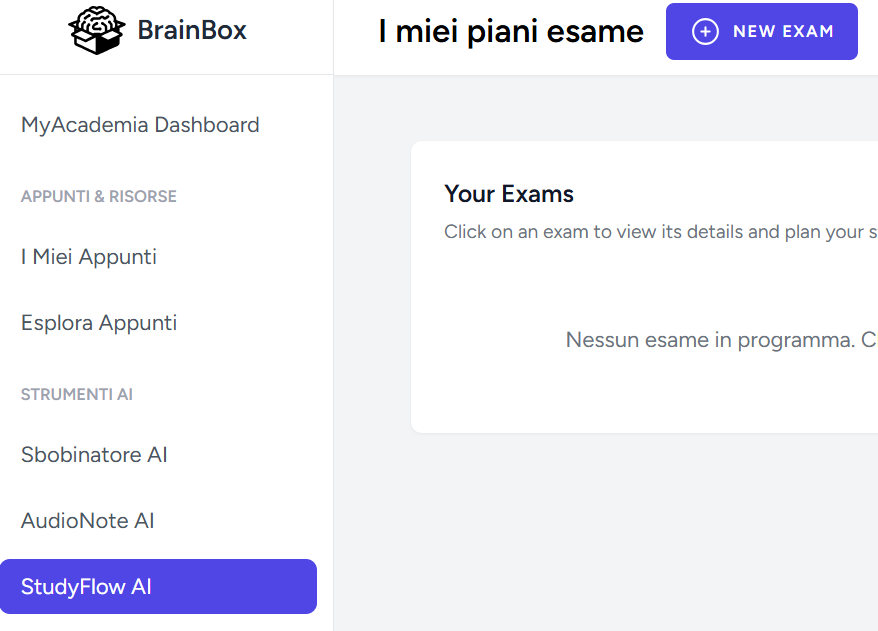
\includegraphics[width=6.5cm]{Screenshots/foglio2/problema023.png}\hspace*{\fill}
    \vspace{10pt}
    \\
    \hline
    \textbf{Nome del valutatore} & Legati, Kharef \\
    \hline
  \end{tabular}
\end{table}

% Problema \getNumeroProblema
\begin{table}[htbp]
  \centering
  \renewcommand{\arraystretch}{1.5}
  \begin{tabular}{|>{\raggedright\arraybackslash}p{7.5cm}|>{\raggedright\arraybackslash}p{7.5cm}|}
    \hline
    \rowcolor{green!30}
    \multicolumn{2}{|c|}{\textbf{Problema \getNumeroProblema}} \\
    \hline
    \textbf{Descrizione} & Nella pagina ”StudyFlow AI”, il bottone ”NEW EXAM” si trova in un punto poco funzionale. \\
    \hline
    \textbf{Pagina del sito} & Dashboard - StudyFlow AI \\
    \hline
    \textbf{Principi violati} & 4 (Assicurare consistenza); 7 (Visualizzare tutte e sole le informazioni necessarie) \\
    \hline
    \textbf{Grado di severità} & 1 (Problema accessorio) \\
    \hline
    \textbf{Screen} &
    \vspace{10pt}
    \hspace*{\fill}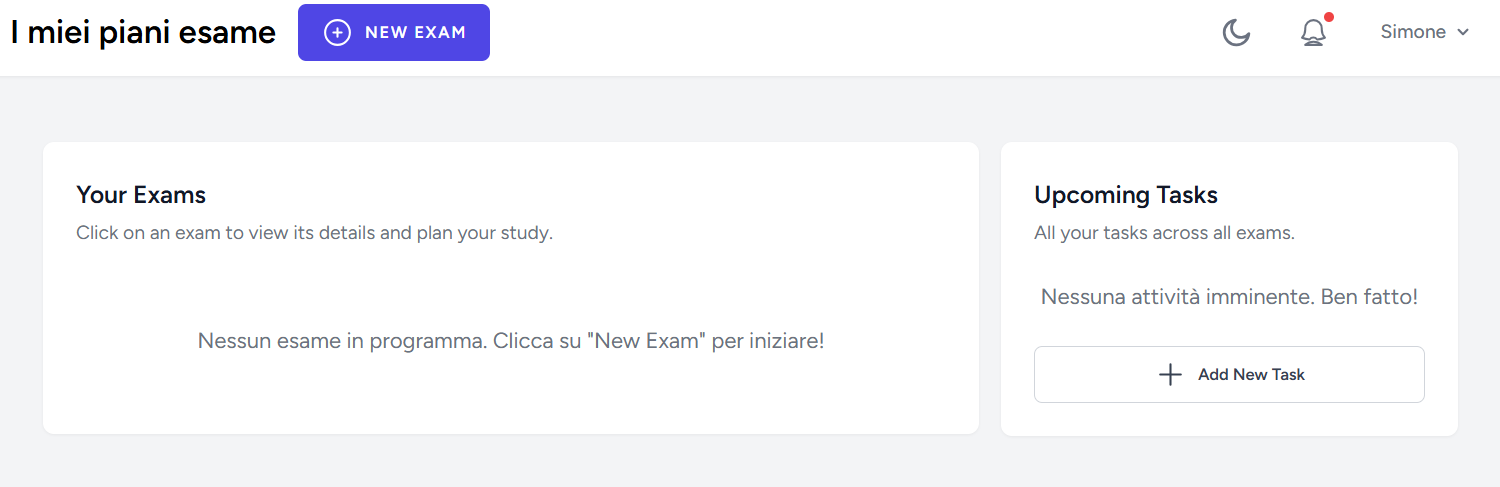
\includegraphics[width=6.5cm]{Screenshots/foglio2/problema024.png}\hspace*{\fill}
    \vspace{10pt}
    \\
    \hline
    \textbf{Nome del valutatore} & Legati \\
    \hline
  \end{tabular}
\end{table}

% Problema \getNumeroProblema
\begin{table}[htbp]
  \centering
  \renewcommand{\arraystretch}{1.5}
  \begin{tabular}{|>{\raggedright\arraybackslash}p{7.5cm}|>{\raggedright\arraybackslash}p{7.5cm}|}
    \hline
    \rowcolor{green!30}
    \multicolumn{2}{|c|}{\textbf{Problema \getNumeroProblema}} \\
    \hline
    \textbf{Descrizione} & Nella pagina ”StudyFlow AI”, il bottone ”NEW EXAM”, a differenza degli altri pulsanti di quel tipo, è scritto in maiuscolo. \\
    \hline
    \textbf{Pagina del sito} & Dashboard - StudyFlow AI \\
    \hline
    \textbf{Principi violati} & 4 (Assicurare consistenza) \\
    \hline
    \textbf{Grado di severità} & 1 (Problema accessorio) \\
    \hline
    \textbf{Screen} &
    \vspace{10pt}
    \hspace*{\fill}
\includegraphics[width=6.5cm]{Screenshots/foglio2/problema025.png}\hspace*{\fill}
    \vspace{10pt}
    \\
    \hline
    \textbf{Nome del valutatore} & Legati \\
    \hline
  \end{tabular}
\end{table}

% Problema \getNumeroProblema
\begin{table}[htbp]
  \centering
  \renewcommand{\arraystretch}{1.5}
  \begin{tabular}{|>{\raggedright\arraybackslash}p{7.5cm}|>{\raggedright\arraybackslash}p{7.5cm}|}
    \hline
    \rowcolor{green!30}
    \multicolumn{2}{|c|}{\textbf{Problema \getNumeroProblema}} \\
    \hline
    \textbf{Descrizione} & La pagina ”StudyFlow AI” presenta contenuti in inglese. \\
    \hline
    \textbf{Pagina del sito} & Dashboard - StudyFlow AI \\
    \hline
    \textbf{Principi violati} & 2 (Adeguare il sistema al mondo reale); 4 (Assicurare consistenza) \\
    \hline
    \textbf{Grado di severità} & 2 (Problema secondario) \\
    \hline
    \textbf{Screen} &
    \vspace{10pt}
    \hspace*{\fill}
\includegraphics[width=6.5cm]{Screenshots/foglio2/problema027.png}\hspace*{\fill}
    \vspace{10pt}
    \\
    \hline
    \textbf{Nome del valutatore} & Legati, Rinaldi \\
    \hline
  \end{tabular}
\end{table}

% Problema \getNumeroProblema
\begin{table}[htbp]
  \centering
  \renewcommand{\arraystretch}{1.5}
  \begin{tabular}{|>{\raggedright\arraybackslash}p{7.5cm}|>{\raggedright\arraybackslash}p{7.5cm}|}
    \hline
    \rowcolor{green!30}
    \multicolumn{2}{|c|}{\textbf{Problema \getNumeroProblema}} \\
    \hline
    \textbf{Descrizione} & Le interfacce degli strumenti AI ("Sbobinatore AI" e "Generatore AudioNote") non forniscono un feedback chiaro e persistente sullo stato di avanzamento del processo. \\
    \hline
    \textbf{Pagina del sito} & Dashboard - Sbobinatore AI / AudioNote AI  \\
    \hline
    \textbf{Principi violati} & 1 (Far vedere lo stato del sistema) ; 3 (Controllo dell’utente e libertà) \\
    \hline
    \textbf{Grado di severità} & 3 (Problema rilevante)  \\
    \hline
    \textbf{Nome del valutatore} & Kharef \\
    \hline
  \end{tabular}
\end{table}

% Problema \getNumeroProblema
\begin{table}[htbp]
  \centering
  \renewcommand{\arraystretch}{1.5}
  \begin{tabular}{|>{\raggedright\arraybackslash}p{7.5cm}|>{\raggedright\arraybackslash}p{7.5cm}|}
    \hline
    \rowcolor{green!30}
    \multicolumn{2}{|c|}{\textbf{Problema \getNumeroProblema}} \\
    \hline
    \textbf{Descrizione} & Le pagine principali ("I Miei Appunti", "Esplora Appunti"), quando vuote, mostrano un semplice messaggio testuale ("Nessun documento"). Questo "empty state" non guida l'utente né lo invita a compiere l'azione primaria per popolare la sezione (es. "Carica il tuo primo appunto!"). \\
    \hline
    \textbf{Pagina del sito} & Dashboard \\
    \hline
    \textbf{Principi violati} & 1 (Far vedere lo stato del sistema); 9 (Permettere all’utente di correggere gli errori e non solo di rilevarli) \\
    \hline
    \textbf{Grado di severità} & 2 (Problema secondario)  \\
    \hline
    \textbf{Screen} &
    \vspace{10pt}
    \hspace*{\fill}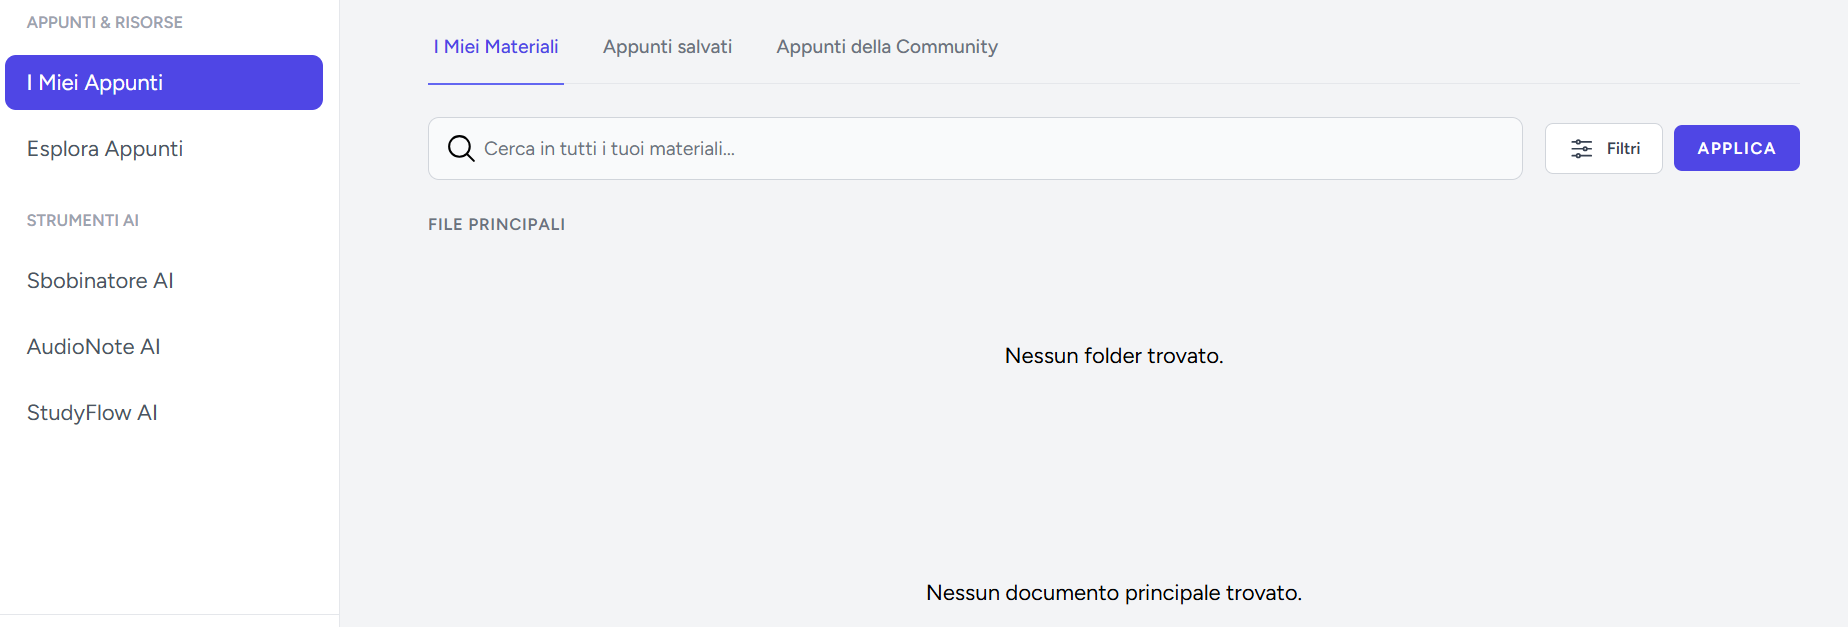
\includegraphics[width=6.5cm]{Screenshots/foglio2/problema029.png}\hspace*{\fill}
    \vspace{10pt}
    \\
    \hline
    \textbf{Nome del valutatore} & Kharef \\
    \hline
  \end{tabular}
\end{table}
